\documentclass[12pt]{article}
\setlength{\oddsidemargin}{0in}
\setlength{\evensidemargin}{0in}
\setlength{\textwidth}{6.5in}
\setlength{\parindent}{0in}
\setlength{\parskip}{\baselineskip}

\usepackage{amsmath,amsfonts,amssymb}
\usepackage{graphicx}
\usepackage{fancyhdr}
\usepackage{hyperref}
\usepackage{color}
\usepackage{blindtext}
\usepackage{subcaption}

\pagestyle{fancy}


\begin{document}
\title{Predicting the Outcome of a UFC Fight Based On the Fighting Styles, Countries, and Training Camps of Both Fighters}
\date{December, 17,  2018}
\author{Nikolai Alexander}
\maketitle

\section{Introduction}

Fight prediction has always been a major part of professional combat sports from the notorious bout between Joe Frazier and Muhammad Ali in 1971, to the epic reign of 175 lbs Brazillian Jiu Jitsu  protege Royce Gracie over the 200+ lbs titans of the early UFC days, to the earthshattering upset where Holly Holms knocked out Ronda Rousey with a head kick in 2015. Many people make a living off of predicting sports outcomes, with the Nevada Sportsbooks bringing in $\$248.8$ million dollars in 2017. However, failed predictions have led to some major upsets in history. For example, Conner McGregor had a $-400$ odds advantage to Nate Diaz ($+300$) for their first bout in 2015. Though, Nate Diaz secured a round 2 submission via rear naked choke after demonstrating a dominating performance against the seemingly invincible featherweight, tripling the wealth of gamblers who bet on his side.

The algorithm used in this project predicts the outcome of a UFC fight based on the age, height, training camp, country, base fighting style, win percentages, and overall professional experience of each of the two fighters. The dataset I used consists of every UFC bout to ever take place between 1993 and 2016 and the statistics of each fighter. Overall, the prediction algorithm produced a test accuracy of $58.1\%$, which was not ideal; however, considering the amount of probability that takes place in a fight, it was deemed acceptable.


\section{Dataset and Preprocessing}

The raw data was found in a \emph{reddit.com} post, where a redditor scraped all fight data from the UFC off of \emph{sherdog.com}. The raw data consisted of two datasets - one of all UFC fights from 1993 to 2016, and the other of all mixed martial artists to ever compete in the UFC. The dataset required quite a bit of annotation and preprocessing before use in the prediction model. First, the base fighting style of each fighter (either the first style the fighter mastered or the style they rely on the most) was manually researched and annotated from \emph{wikipedia.com}, \emph{tapology.com}, and \emph{ufc.com} for all $1,526$ fighters. Additionally, the win, loss, and win percentage of each fighter were scraped from \emph{sherdog.com} with a python script.

The feature selection and feature engineering processes were the dominant part of this project. The two datasets were combined into one dataset, placing the statistics from each fighter into their respective fights in the fight dataset. Since the data was mostly categorical (association, country, base style), the features needed to be converted to some sort of numerical scale. The first thing I observed was the histograms of three of the features: country, association, and base style.

\begin{figure}[h!]
\centering
\begin{subfigure}{.5\textwidth}
  \centering
  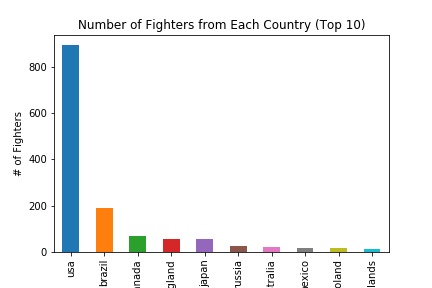
\includegraphics[width=.85\linewidth]{country_hist.png}
  \label{fig:sub1}
\end{subfigure}%
\begin{subfigure}{.5\textwidth}
  \centering
  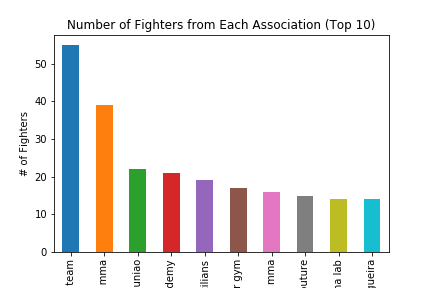
\includegraphics[width=.85\linewidth]{gym_hist.png}
  \label{fig:sub2}
\end{subfigure}
\begin{subfigure}{.5\textwidth}
  \centering
  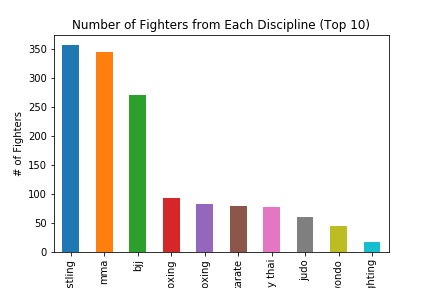
\includegraphics[width=.85\linewidth]{style_hist.png}
  \label{fig:sub1}
\end{subfigure}%
\label{fig:test}
\end{figure}

I decided to convert each of features into numerical data using their overall win rates. However, I needed to find a way to weigh them properly, as a gym with a 1-0 record would have a $100\%$ win rate, though a gym with a 19-1 record would have a $95\%$ win rate. To give the categories with more fights a slight advantage, I decided to normalize the number of fighters from each country, association, and base\_style and add those values to the features' respective win rates.

After applying these scores to the fighter data, I combined the fighter data with the fight data, creating an entirely new dataset. Each instance in the dataset is a fight between two mixed martial artists. The features consist of the names of both fighters, their ages, heights, win rates, total fights, and the gym scores, country scores, and style scores calculated through feature engineering. The outcome in the dataset is the result of the fight, with $1$ meaning the first fighter won, $-1$ meaning the second fighter 2 won, and $0$ meaning a draw or no contest. I then applied a min-max scalar transform on the features to normalize the weights of all features.

Finally, before calulating different prediction models. I split the data into three sets: training ($64\%$), validation ($16\%$), and testing ($20\%$).


\section{Prediction}

For the prediction, I tested 3 models using the training and validation data. The began with a linear classification, using Logistic Regression. I made $7$ tests, adjusting alpha logrithmicly between $10^{-4}$ and $100$.

\begin{figure}[h!]
\centering
\begin{subfigure}{.5\textwidth}
  \centering
  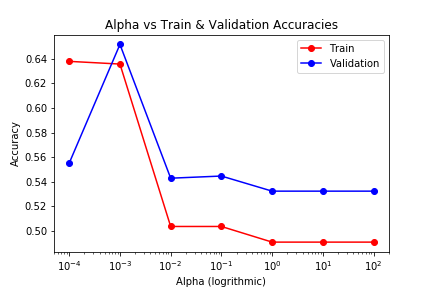
\includegraphics[width=.88\linewidth]{logreg_plot.png}
  \label{fig:sub1}
\end{subfigure}%
\label{fig:test}
\end{figure}

I found that the highest validation accuracy was $65.1\%$ when alpha was equal to $10^{-3}$. However, I figured there must be a better method of prediction.

The next method I explored was using a non-linear classifier, as mixed martial arts is a complex sport involving many different factors. I decided a Support Vector Classification with an RBF kernal was the best approach to the problem. To get a rough idea of the accuracy of the algorithm, I tested 8 different models, adjusting the penalty parameter C logrithmically between $10^{-4}$ and $1000$.

\begin{figure}[h!]
\centering
\begin{subfigure}{.6\textwidth}
  \centering
  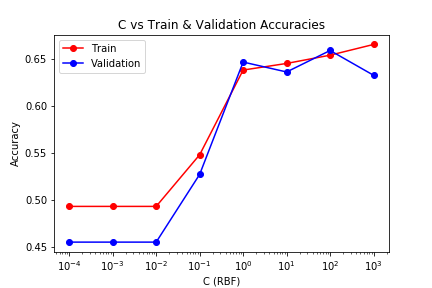
\includegraphics[width=.9\linewidth]{rbf_plot.png}
  \label{fig:sub1}
\end{subfigure}%
\label{fig:test}
\end{figure}

I noticed the rbf model performed the best at $C=100$, and was slightly more accurate than Logrithmic Regression with a validation accuracy of $65.8\%$. 

The third and final prediction method I observed was a Generative Classifier using Naive Bayes. This method performed the worst of the three, with a validation accuracy of $46.6\%$, which was worse than all cases of Logistic Regression, and around the same as the worst case of the Support Vector.

I decided to go with the Support Vector Machine with an RBF kernal and $C=100$, as that performed best out of the three methods. I attempted to tune my prediction model further by testing different kernel coefficients, gamma, for RBF. The coefficient that performed the best was $gamma=10^{-3}$, however, it still performed lower than when gamma was set to 'auto' with a validation accuracy of $64.5\%$, so I decided to leave out of my prediction model.

My final prediction on my test data resulted in a $58.1\%$ accuracy.


\section{Error Analysis}

The prediction model produced the below confusion matrix,

\begin{table}[h!]
\centering
\begin{tabular}{|l|l|l|l|}
\hline
            & \textbf{1} & \textbf{0} & \textbf{-1} \\ \hline
\textbf{1}  & 235        & 0          & 126         \\ \hline
\textbf{0}  & 12         & 0          & 4           \\ \hline
\textbf{-1} & 157        & 0          & 180         \\ \hline
\end{tabular}
\end{table}

There were $404$ predicted wins and a $58.2\%$ accuracy, and only $310$ predicted losses with a $58.1\%$ accuracy. It predicted both wins and losses with approximately the same accuracy, showing that there was not a lot of favoritism towards either outcome. However, it did not once predict a draw or no contest. I believe it failed to predict a draw, since they are very rare, and predicting a no-contest would be the equivalent of predicting whether or not a fighter was caught for using performance enhancing drugs (PEDs), which would require and entirley different dataset.

\section{Conclusion}

Altogether, I believe $58.1\%$, though not ideal, is an acceptable accuracy considering how many random factors fall into the outcome of a fight. Preperation through training camps, effective weight cutting, and the probability of someone landing a lucky shot that will knock their opponent out are difficult things to predict leading up to a fight as they are purely situational. As I believe there is a better prediction model that would perform more accurately than my model, there is a high enough density of upsets throughout the UFC's history to demonstrate that it is really anybody's game. If I were to do this experiment differently, I would add factors such as finishing rate, types of finished (TKO, Submission, KO), and stats such Striking and Grappling Accuracy, Defense, and Significant Strikes, and Ring Control as these all factor into a fighter's performance. However, this information is difficult to legally acquire as it is heavily copywrited by the UFC.

\end{document}